%%%%%%%%%%%%%%%%%%%%%%%%%%%%%%%%%%%%%%%%%
% Beamer Presentation
% LaTeX Template
% Version 1.0 (10/11/12)
%
% This template has been downloaded from:
% http://www.LaTeXTemplates.com
%
% License:
% CC BY-NC-SA 3.0 (http://creativecommons.org/licenses/by-nc-sa/3.0/)
%
%%%%%%%%%%%%%%%%%%%%%%%%%%%%%%%%%%%%%%%%%

%----------------------------------------------------------------------------------------
%	PACKAGES AND THEMES
%----------------------------------------------------------------------------------------

\documentclass{beamer}

\mode<presentation> {

% The Beamer class comes with a number of default slide themes
% which change the colors and layouts of slides. Below this is a list
% of all the themes, uncomment each in turn to see what they look like.

%\usetheme{default}
%\usetheme{AnnArbor}
%\usetheme{Antibes}
%\usetheme{Bergen}
%\usetheme{Berkeley}
%\usetheme{Berlin}
%\usetheme{Boadilla}
%\usetheme{CambridgeUS}
%\usetheme{Copenhagen}
%\usetheme{Darmstadt}
%\usetheme{Dresden}
%\usetheme{Frankfurt}
%\usetheme{Goettingen}
%\usetheme{Hannover}
%\usetheme{Ilmenau}
%\usetheme{JuanLesPins}
%\usetheme{Luebeck}
\usetheme{Madrid}
%\usetheme{Malmoe}
%\usetheme{Marburg}
%\usetheme{Montpellier}
%\usetheme{PaloAlto}
%\usetheme{Pittsburgh}
%\usetheme{Rochester}
%\usetheme{Singapore}
%\usetheme{Szeged}
%\usetheme{Warsaw}

% As well as themes, the Beamer class has a number of color themes
% for any slide theme. Uncomment each of these in turn to see how it
% changes the colors of your current slide theme.

%\usecolortheme{albatross}
%\usecolortheme{beaver}
%\usecolortheme{beetle}
%\usecolortheme{crane}
%\usecolortheme{dolphin}
%\usecolortheme{dove}
%\usecolortheme{fly}
%\usecolortheme{lily}
%\usecolortheme{orchid}
%\usecolortheme{rose}
%\usecolortheme{seagull}
%\usecolortheme{seahorse}
%\usecolortheme{whale}
%\usecolortheme{wolverine}

%\setbeamertemplate{footline} % To remove the footer line in all slides uncomment this line
%\setbeamertemplate{footline}[page number] % To replace the footer line in all slides with a simple slide count uncomment this line

%\setbeamertemplate{navigation symbols}{} % To remove the navigation symbols from the bottom of all slides uncomment this line
}

\usepackage{graphicx} % Allows including images
\DeclareGraphicsExtensions{.pdf,.png,.jpg}
\usepackage{booktabs} % Allows the use of \toprule, \midrule and \bottomrule in tables
\usepackage[skip = 2pt, font=scriptsize]{caption}
\usepackage{subfigure}

%----------------------------------------------------------------------------------------
%	TITLE PAGE
%----------------------------------------------------------------------------------------

\title[RooMCMC]{MCMC fitter for Root} % The short title appears at the bottom of every slide, the full title is only on the title page

\author{Oliver Dahme} % Your name
\institute[UZH] % Your institution as it will appear on the bottom of every slide, may be shorthand to save space
{
University of Zurich \\ % Your institution for the title page
\medskip
\textit{o.dahme@cern.ch} % Your email address
}
\date{\today} % Date, can be changed to a custom date

\begin{document}

\begin{frame}
\titlepage % Print the title page as the first slide
\end{frame}

\begin{frame}
\frametitle{Overview} % Table of contents slide, comment this block out to remove it
\tableofcontents % Throughout your presentation, if you choose to use \section{} and \subsection{} commands, these will automatically be printed on this slide as an overview of your presentation
\end{frame}

%----------------------------------------------------------------------------------------
%	PRESENTATION SLIDES
%----------------------------------------------------------------------------------------

%------------------------------------------------
\section{Introduction} % Sections can be created in order to organize your presentation into discrete blocks, all sections and subsections are automatically printed in the table of contents as an overview of the talk
%------------------------------------------------

\begin{frame}
\frametitle{Monte Carlo Markov Chain}
A Markov Chain is a random process which undergoes several states. \\
From each state there is a probability distribution to change into another state or to stay. \\
Most important is the asumption that every next step just depends on the current state.
\begin{figure}
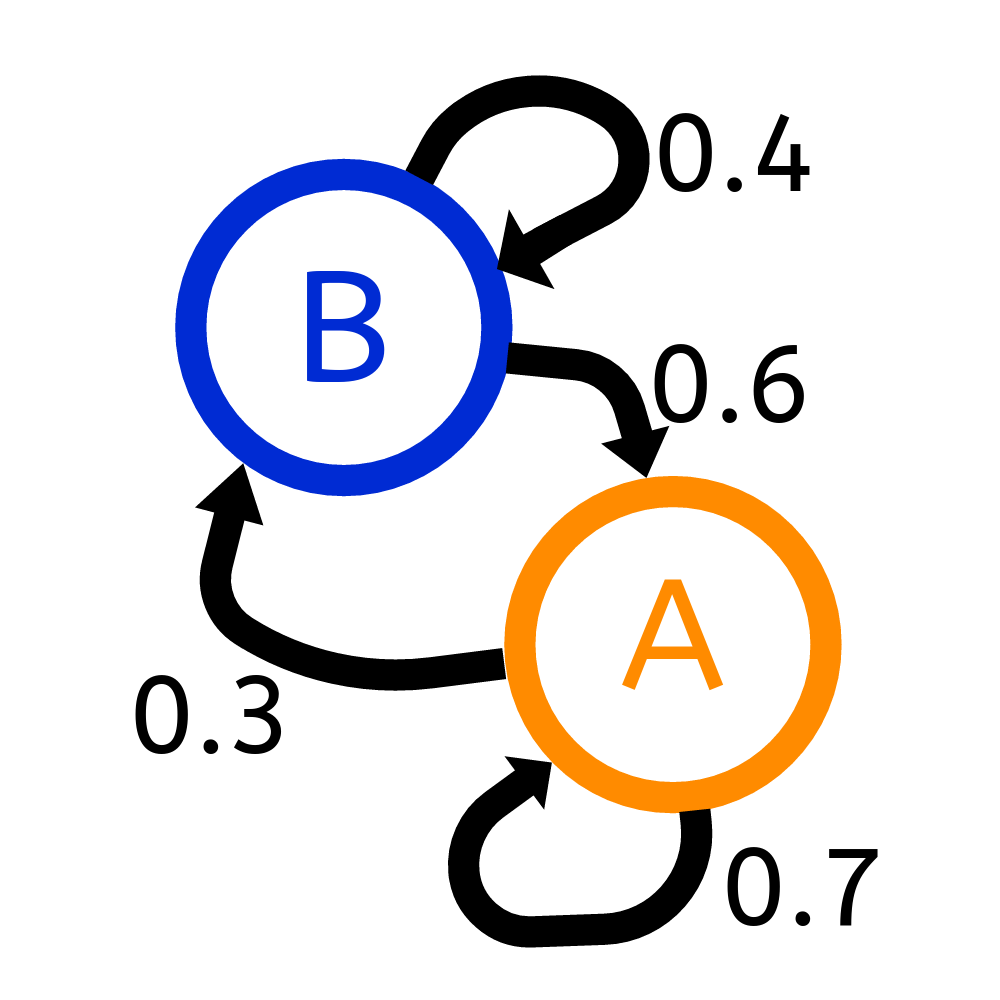
\includegraphics[width=0.3\linewidth]{figures/MCMC_Chain}
\caption{By Joxemai4 - Own work, CC BY-SA 3.0, https://commons.wikimedia.org/w/index.php?curid=10284158}
\end{figure}
\end{frame}

%--------------------------------------------------------------

\begin{frame}
\frametitle{The algorithm}
\begin{figure}
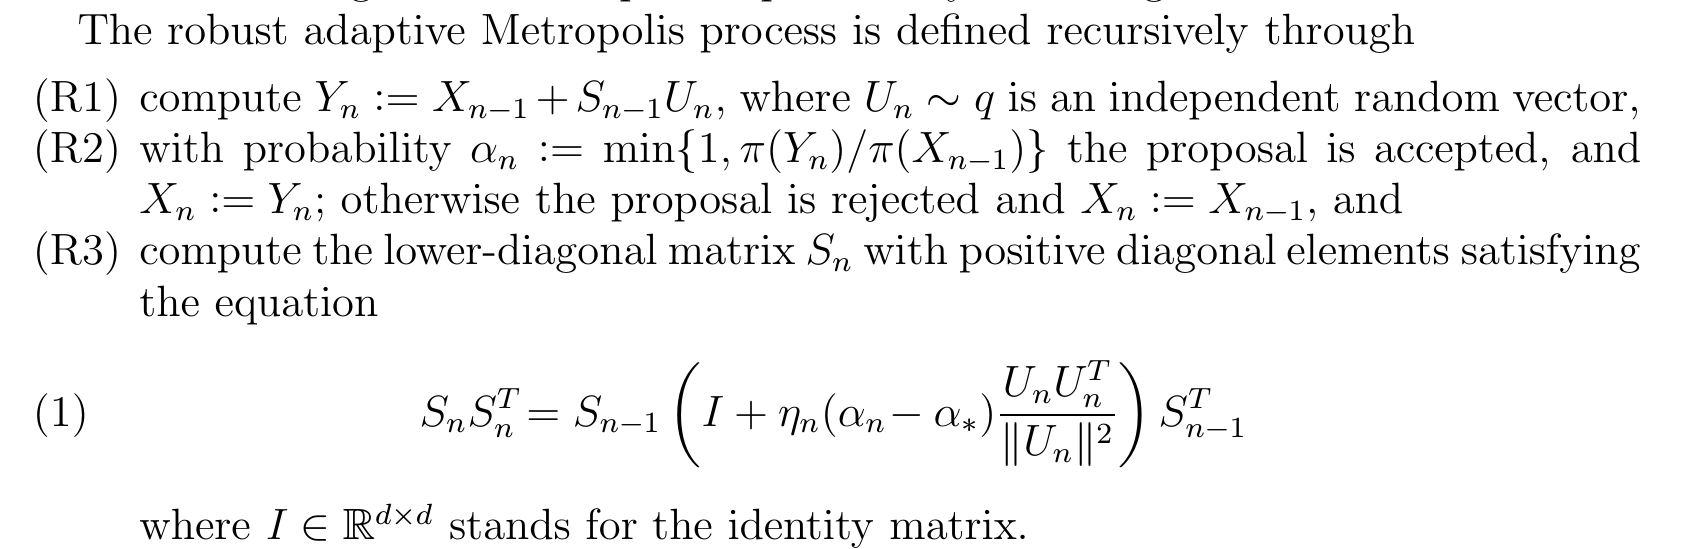
\includegraphics[width=1.0\linewidth]{figures/Metropolis}
\caption{arXiv: 1011.4381v2}
\end{figure}
Here $Y_n$ is the next state and $X_{n-1}$ is the current state. \\
The $S$-maxtrix determs the direction of the next step. \\
It basically depends on the gradient of the function, which leads the walk towards the minimum.
\end{frame}

%---------------------------------------------------------------
\begin{frame}
\frametitle{The algorithm}
Proof of concept: A Metropolis walk (b) has been performed for the Gaus points in (a).\\
\begin{figure}
  \subfigure[1000 Simulated Gaus points, with real mean at 3 and real sigma at 1.5]{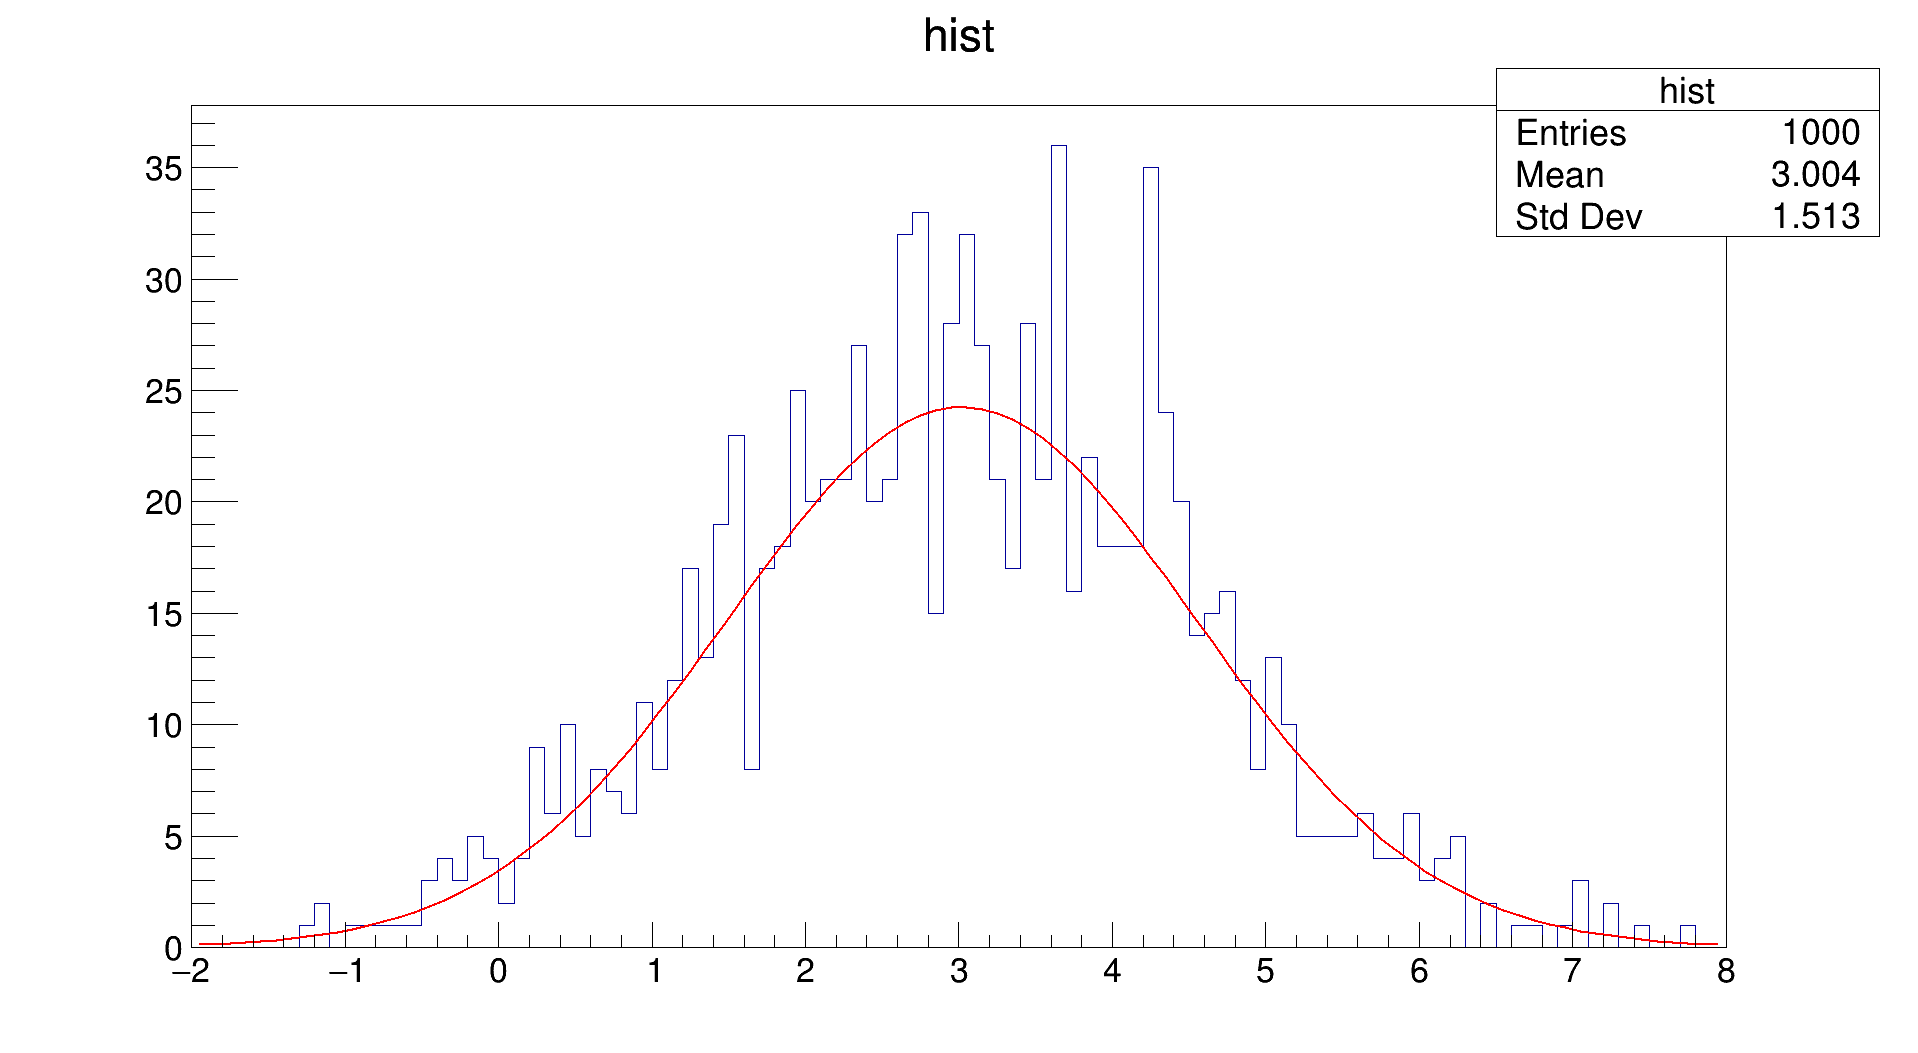
\includegraphics[width=0.49\textwidth]{figures/gauspoints}}
  \subfigure[One Toy of the Metropolis walk]{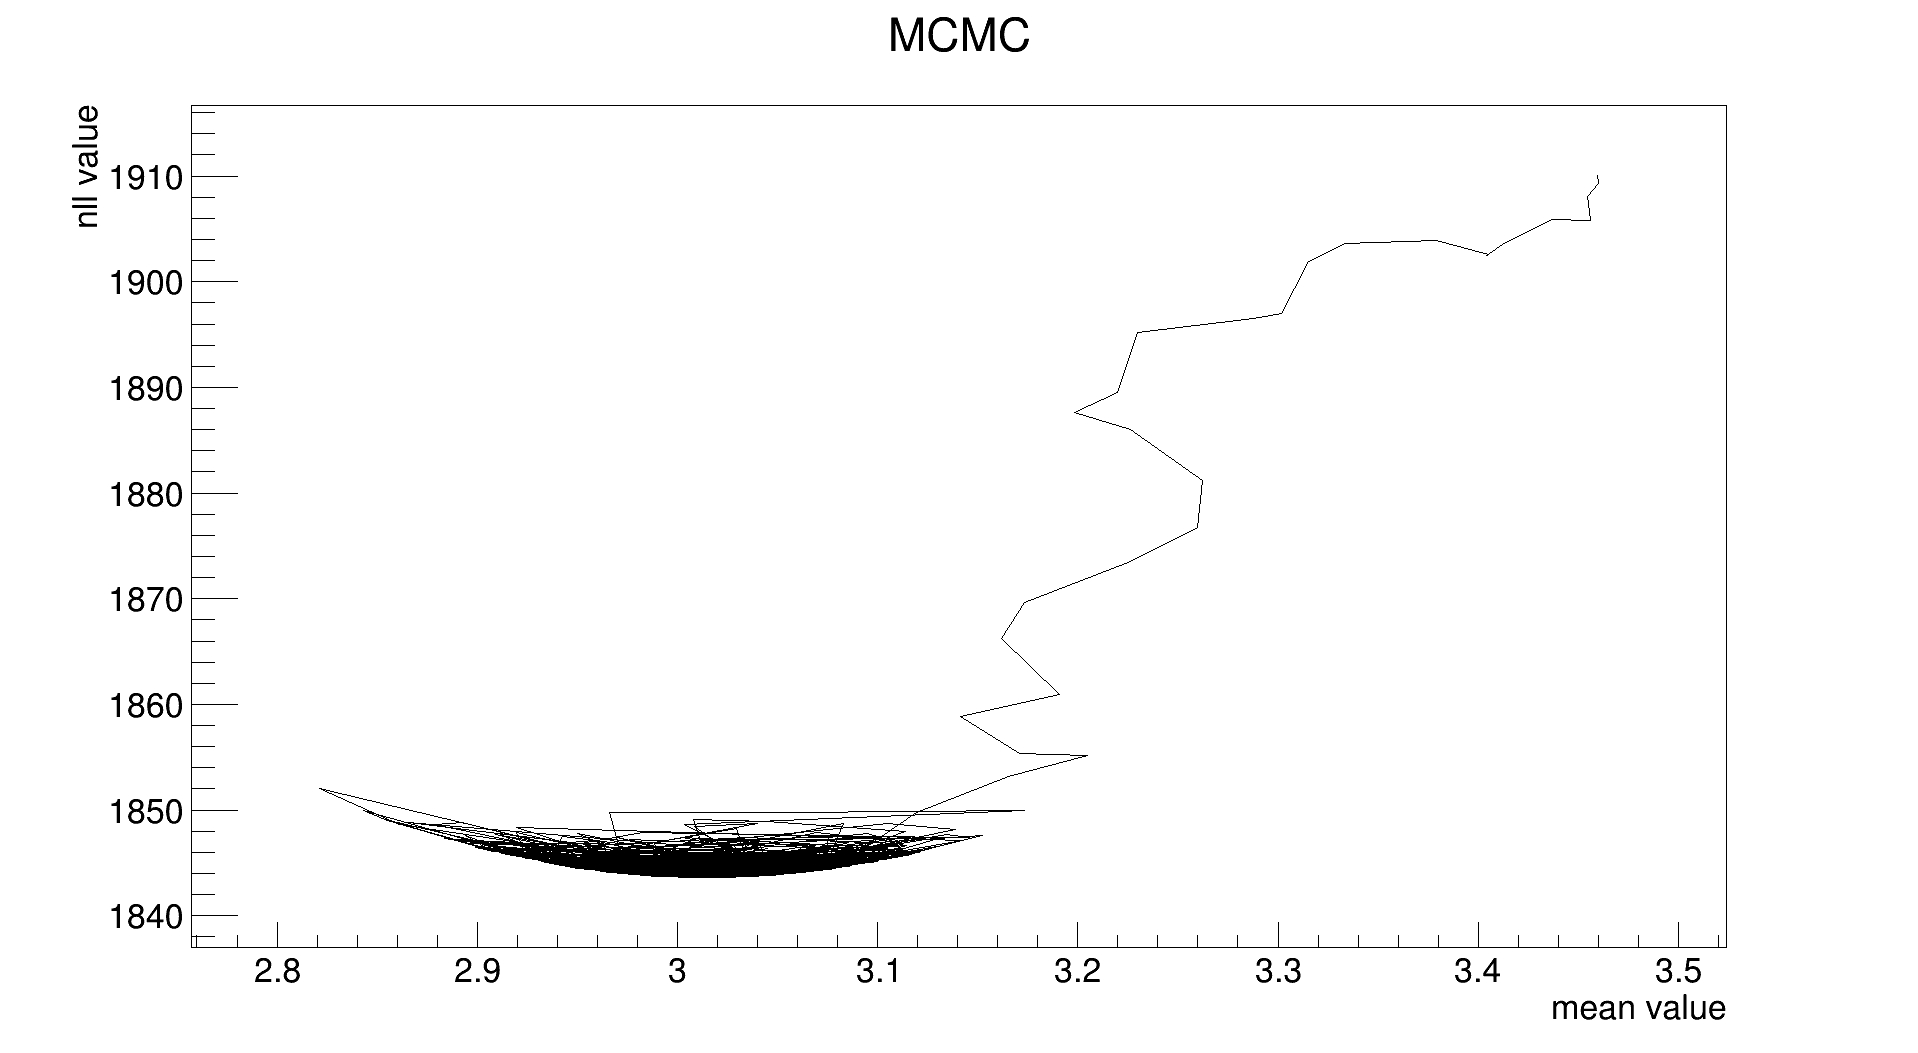
\includegraphics[width=0.49\textwidth]{figures/muprofile}}
\end{figure}
The walk converges towards the minimum. \\
Than the walk starts jumping arround the true value.
\end{frame}


%----------------------------------------------------------------------------------------

\end{document}
